
\subsection{Introduction to cost estimation}

Estimating the cost of a software project is a non trivial task. Many
aspects contribute to determine the effort put in a software project
and relationships among the characteristics of the project team (number
of people, type of organization, ...), the features of the project
itself (complexity) and the environmental influences are typically
intricate and difficult to be estimated with an acceptable degree
of approximation. Therefore often we rely on the \emph{experience-based
techniques} where the estimation is made by an experienced manager
on the basis on the past projects and the application domain, sometimes
this task is performed by a team of experts (community-based estimation).
If no experts are available, or the domain of the application in too
specific only \emph{algorithmic cost modeling }is allowed. Those techniques
are based on a formulated approach to compute the project effort based
on estimates of product attributes. We will adopt the \emph{Function
Points} technique that was proposed by Allan Albrecht at IBM in 1965
and then COCOMOII that was developed around '80 based on the statistical
analysis performed by Barry Boehn on the basis on many real projects
coming from various domains.


\subsection{Function points approach}

There is an underlying hypothesis behind function points: the dimension
of software can be characterized by \emph{abstraction}. Therefore
after the architectural design (early in the project life cycle),
when the product model is almost clear, a rough evaluation of the
size of the software can be performed. Albrecht’s method identifies
and counts the number of function types within the software (actually
its model), those types constitutes the “external representation”
of an application, that is, its functionality as defined from an abstract
point of view. The types of functionalists are the following:
\begin{itemize}
\item \emph{Internal Logical File} (ILF): homogeneous set of data used and
managed by the application.
\item \emph{External Interface File} (EIF): homogeneous set of data used
by the application but generated and maintained by other applications.
\item \emph{External Input}: elementary operation to elaborate data coming
form the external environment.
\item \emph{External Output:} elementary operation that generates data for
the external environment; it usually includes the elaboration of data
from logic files.
\item \emph{External Inquiry}: elementary operation that involves input
and output, without significant elaboration of data from logic files.
\end{itemize}
The measure of the size of the software is given by the weighed average
of the function points (number of each function type listed above),
according to the following predefined table.\bigskip{}


\begin{center}
\begin{tabular}{>{\raggedright}p{5cm}|>{\centering}p{2cm}|>{\centering}p{2.5cm}|>{\centering}p{2cm}}
\hline 
\multirow{2}{5cm}{\textbf{Function type}} & \multicolumn{3}{>{\centering}p{7cm}}{\textbf{Weight}}\tabularnewline
\cline{2-4} 
 & \emph{Simple} & \emph{Average} & \emph{Complex}\tabularnewline
\hline 
\emph{EI (External Inputs)} & 3 & 4 & 6\tabularnewline
\hline 
\emph{EO (External Outputs)} & 4 & 5 & 7\tabularnewline
\hline 
\emph{EQ (External Inquiries)} & 3 & 4 & 6\tabularnewline
\hline 
\emph{ILF (Internal Logical Files)} & 7 & 10 & 15\tabularnewline
\hline 
\emph{ELF (External Logical Files)} & 5 & 7 & 10\tabularnewline
\hline 
\end{tabular}
\par\end{center}

\bigskip{}


The resulting sum is called UFP (Unadjusted Function Points). This
value can be further manipulated with the ``adjustment'' formula
to get an estimation of the effort, however the result is usually
little significant, therefore it is suggested to use the UFP in combination
with other effort estimation algorithms like COCOMO II. 


\subsection{Function point count}

In this section we present the function point count; for each type
of functionality we list the ones we have identified within the myTaxiService
system with the corresponding complexity and a rational for our choice.
According to the Albrecht definition, this process is performed by
abstraction therefore the main resource is the RASD in particular
the high level class diagram for the logical files and the use cases
for the inputs, outputs and inquiries.


\subsubsection{ILF (Internal logical files)}

The application includes a number of ILFs that will be used to store
information about:
\begin{itemize}
\item \emph{passengers}, in particular username, password, lastname, firstname,
email and address;
\item \emph{taxi drivers}, in particular username, password, firstname and
lastname;
\item \emph{taxis}, in particular the plate number, the code, the number
of seats and the current state;
\item \emph{requests}, in particular the date and time in which the request
is sent, the number of passengers, the location (geographical coordinates
and the address) of the passenger, possibly the waiting time and the
taxis assigned to the request itself;
\item \emph{reservations}, in particular the date and time in which the
request is sent, the number of passengers, the location (geographical
coordinates and the address) of both origin and destination and the
corresponding attached request;
\item \emph{zones}, in particular the name of the zone, the estimation of
the requests per minute and the adjacency relation among zones;
\item \emph{queues}: in particular the proper size of the queue (and also
the minimum and maximum number of taxis allowed) and the taxis belonging
to the queue with the corresponding position.
\end{itemize}
Each of these entities has a simple structure with a limited number
of fields except for the queue which requires a quite articulated
structure to manage positions and sizes of queues. Thus, we select
medium complexity for the latter and simple for the other ones. 

\[
ILF=6\cdot7+1\cdot10=52FPs
\]



\subsubsection{ELF (External logical files)}

myTaxiService has to interact with external systems, in particular
with the GPS and the GoogleMaps API therefore we can identify the
following ELFs:
\begin{itemize}
\item \emph{Address validation }requires the interaction with the GoogleMaps
API in order to check whether a string typed by the user corresponds
to a valid address.
\item \emph{Coordinate/Address translation} requires the interaction with
the GoogleMaps API in order to convert a coordinate retrieved by the
GPS into an address and viceversa.
\item \emph{Travelling time }requires the interaction with the GoogleMaps
API in order to compute the waiting time.
\item \emph{Passenger's geographic coordinates} requires the interaction
with the GPS system installed on the passenger smartphone or with
the browser geolocalization to retrieve the passenger's position.
\item \emph{Taxi geographic coordinates} requires the interaction with the
GPS installed on each taxi in order to find the position of the taxi
itself.
\end{itemize}
All those data items are very compact and they share the same simple
structure, so a simple complexity should be appropriate. 

\[
ELF=5\cdot5=25FPs
\]



\subsubsection{EI (External inputs)}

Since myTaxiService is an application characterized of having a high
degree of interaction with the final user, we can identify the following
EI.
\begin{itemize}
\item \emph{Registration}: this function requires the exchange of a relevant
amount of information (username, password, lastname, firstname, email
and address), in addition some checks has to be performed (like check
that the username is not already used), so we can consider medium
complexity with a contribution of 4 FPs.
\item \emph{Login/Logout}: this function is standard and requires exchange
of basic structured information and simple operations, so it can be
considered simple with a contribution of 3 FPs.
\item \emph{Request}: this function requires the insertion of some data
(like address), the interaction with external systems (like GPS and
GoogleMaps API) and with the DBMS, therefore it can be considered
complex with a contribution of 6 FPs.
\item \emph{Taxi selection}: this function requires non trivial elaborations
related to the algorithm used to select the taxis to fulfill a request/reservation;
it requires interaction with the DBMS and external systems therefore
it can be considered complex with a contribution of 6 FPs.
\item \emph{Taxi queue management}: this function requires the execution
of the algorithm described in the design document for the taxi movement,
in addition it requires to interact with external systems and the
DBMS therefore it can be considered complex with a contribution of
6 FPs.
\item \emph{Reservation}: this function requires interaction with the DBMS
and with external systems, it has also to instantiate a new request
associated to the reservation and to perform validity checks on the
inserted data, therefore it can be considered complex with a contribution
of 6 FPs.
\item \emph{Modify reservation}: this function can be considered an extension
of Reservation, adding a small new functionality, therefore it can
be considered simple with a contribution of 3 FPs.
\item \emph{Cancel reservation}: this function can be considered an extension
of Reservation, adding a small new functionality, therefore it can
be considered simple with a contribution of 3 FPs.
\item \emph{Request evaluation}: this function requires to interact with
the TMA and the analysis of the taxi queues, so it can be considered
medium complexity with a contribution of 4 FPs.
\item \emph{Inform about availability}: this function requires to check
some conditions to validate the state changing of the taxi driver,
it can be considered medium complexity with a contribution of 4 FPs.
\item \emph{Insert phone request}: this function is just reduced to Request
therefore it can be considered simple with a contribution of 3 FPs.
\end{itemize}
\[
EI=4\cdot3+3\cdot4+4\cdot6=48FPs
\]



\subsubsection{EO External output}

The only external outputs generated by the myTaxiService are:
\begin{itemize}
\item \emph{Movement notification: }that function is performed by the system
to communicate to the taxi driver the notification of the movement,
since it requires the evaluation of the taxi queues it can be considered
medium complexity with a contribution of 5 FPs.
\item \emph{Request notification: }this function is performed in order to
communicate to the taxi driver a request to be carried out, it requires
only to send information about the address of the passenger therefore
it can be considered simple with a contribution of 4 FPs.
\end{itemize}
\[
EI=1\cdot4+1\cdot5=9FPs
\]



\subsubsection{EQ External inquiries}

We identified the following EQs.
\begin{itemize}
\item \emph{Visualize request info}: this function allows passenger, both
registered or not, to visualize the information about the last request
including waiting time and the number of incoming taxi.
\item \emph{Visualize previous reservations}: this function allows registered
passengers to visualize the previous sent reservations.
\item \emph{Visualize previous requests (taxi driver)}: this function allows
the taxi driver to visualize the previous requests carried out.
\end{itemize}
All these functions requires the interaction with the DBMS therefore
they can be considered medium complexity.

\[
EI=3\cdot4=12FPs
\]



\subsubsection{UFP Unadjusted Function Points count}

Here we summarize the number of function points identified in every
category and we provide the UFP (Unadjusted Function Points count)
which could possibly be adjusted to take into account organizational
aspects and get an estimation of the effort, however this approach
is typically very imprecise therefore we will use UFP in combination
with the COCOMO approach.

\bigskip{}


\noindent \begin{center}
\begin{tabular}{>{\raggedright}p{5cm}|>{\centering}p{1.5cm}}
\hline 
\multicolumn{1}{l|}{\textbf{Function type}} & \textbf{FPs}\tabularnewline
\hline 
\hline 
\emph{ILF (Internal Logical Files)} & 52\tabularnewline
\hline 
\emph{ELF (External Logical Files)} & 25\tabularnewline
\hline 
\emph{EI (External Inputs)} & 48\tabularnewline
\hline 
\emph{EO (External Outputs)} & 9\tabularnewline
\hline 
\emph{EQ (External Inquiries)} & 12\tabularnewline
\hline 
\end{tabular}
\par\end{center}

\bigskip{}


Thus, we get at the end the value of UFP

\textbf{
\[
UFP=ILF+ELF+EI+EO+EQ=146FPs
\]
}

Here we provide an histogram representing the number of function points
for each category.

\begin{figure}[H]
\noindent \begin{centering}
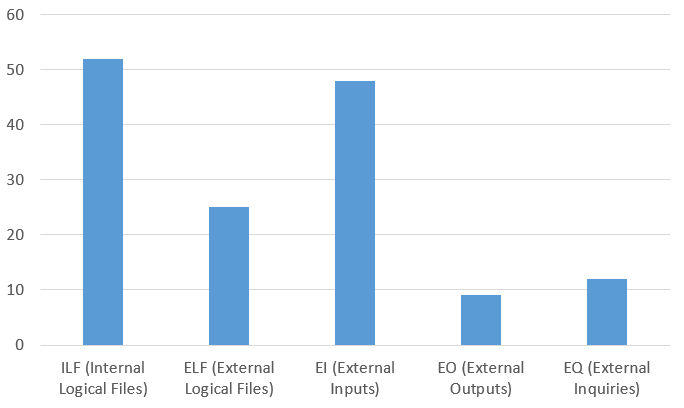
\includegraphics[scale=0.7]{function-points/fp}
\par\end{centering}

\protect\caption{Function Points Histogram}
\end{figure}



\subsection{Lines of code count}

The Unadjusted Function Points (UFP) can be used to provide an estimation
of the number of lines of code (SLOC) of the final project according
to the specific implementation language chosen. Instead of referring
to the ``traditional'' table proposed by Jones 1996 for the conversion
factor, which by the way does not include a value for JEE, we adopt
the more recent Function Points Language Table proposed in {[}7{]}.
myTaxiService is intended to be implemented with JEE, the table provides
a range for the conversion factor SLOC/FP

\bigskip{}


\noindent \begin{center}
\begin{tabular}{>{\centering}p{2cm}|>{\centering}p{2cm}|>{\centering}p{2cm}|>{\centering}p{2cm}|>{\centering}p{2cm}}
\hline 
\textbf{Language} & \emph{Average} & \emph{Median} & \emph{Low} & \emph{High}\tabularnewline
\hline 
J2EE & 46 & 49 & 15 & 67\tabularnewline
\hline 
\end{tabular}
\par\end{center}

\bigskip{}


Not having precise information about the complexity of the implementation
we think an average value should be proper, so $SLOC/FP=46$ and we
get the value of SLOC.

\[
SLOC=SLOC/FP\cdot UFP=46\cdot146=6716
\]


Notice that this value does not capture, for the most part, the client
side of the application and the web server. Since both PMA, TMA and
web server do not perform meaningful functions at requirement level
but just auxiliary functions they are not highlighted in the function
points count, however from an implementation point of view they might
require a relevant effort.
